\documentclass[letterpaper]{ieeeconf}
\usepackage{amsmath,amssymb}
\usepackage{cite}
\usepackage{amsthm,amsfonts}
\usepackage{graphicx}
\usepackage[hidelinks]{hyperref}
\usepackage[ruled,linesnumbered]{algorithm2e}
\usepackage{tikz}
\usepackage{lipsum}
\usepackage{MnSymbol}
%\usepackage{todonotes}

\def\spoke#1#2{
\begin{scope}[shift={#1}, rotate=#2]
    \draw[thick] (0,-.15) -- (0,-1);
\end{scope}
}
\providecommand{\red}[1]{\textcolor{red}{#1}}
\providecommand{\nf}[1]{\normalfont #1}
\providecommand{\R}{\ensuremath \mathbb{R}}
\providecommand{\N}{\ensuremath \mathbb{N}}
\providecommand{\ip}[1]{\ensuremath \left\langle #1\right\rangle}
\newtheorem{lemma}{Lemma}
\theoremstyle{remark}
\newtheorem{remark}{Remark}
\theoremstyle{definition}
\newtheorem{defn}{Definition}
\newtheorem{assump}{Assumption}
\newtheorem{example}{Example}
\newcommand{\Ram}[1]{\textcolor{red}{#1}}

\newcommand*\circled[1]{\tikz[baseline=(char.base)]{
            \node[shape=circle,draw,inner sep=.pt] (char) {#1};}}


\title{Convex Computation of the Reachable Set for Hybrid Systems with Parametric Uncertainty}

\author{Shankar Mohan and Ram Vasudevan \vspace*{-0.75cm}
 \thanks{S. Mohan is with the Department of Electrical Engineering and Computer Science, University of Michigan, Ann Arbor, MI 48109
{\scriptsize \texttt{elemsn@umich.edu}}}
 \thanks{R. Vasudevan is with the Department of Mechanical Engineering, University of Michigan, Ann Arbor, MI 48109
{\scriptsize \texttt{ramv@umich.edu}}}% <-this % stops a space
}

\begin{document}
\maketitle
  \begin{abstract}
  	To verify the correct operation of systems, engineers need to determine the set of configurations of a dynamical model that are able to safely reach a specified configuration under a control law.
	Unfortunately, constructing models for systems interacting in highly dynamic environments is difficult.
	This paper addresses this challenge by presenting a convex optimization method to efficiently compute the set of configurations of a polynomial hybrid dynamical system that are able to safely reach a user defined target set despite parametric uncertainty in the model.
	This class of models describes, for example, legged robots moving over uncertain terrains.
	The presented approach utilizes the notion of occupation measures to describe the evolution of trajectories of a nonlinear hybrid dynamical system with parametric uncertainty as a linear equation over measures whose supports coincide with the trajectories under investigation.
	This linear equation with user defined support constraints is approximated with vanishing conservatism using a hierarchy of semidefinite programs each of which is proven to compute an outer approximation to the set of initial conditions that can reach the user defined target set safely in spite of uncertainty.
	The efficacy of this method is illustrated on a pair of nonlinear systems with parametric uncertainty.
  \end{abstract}
  \section{Introduction}

Computing the set of configurations that are able to safely reach a desired configuration is critical to ensuring the correct performance of a system in dynamic environments where deviations from planned behavior are to be expected.
Many methods have been proposed to efficiently compute this set that is generally referred to as the \emph{backwards reachable set} for deterministic systems.
Unfortunately, the effect of intermittent contact with the world, especially in fluctuating environments, is demanding to model deterministically.
A roboticist, for example, may be tasked with ensuring that a control for a legged robot beginning from an initial configuration is able to safely reach a desired goal; however, limitations in sensing or environment variability may render exact modeling of terrain height or friction impossible.
The development of numerical tools to tractably compute the backwards reachable set of dynamical systems undergoing contact, or \emph{hybrid dynamical systems}, with parametric uncertainty while providing systematic guarantees has been challenging due to the difficulty of efficiently accounting for the uncertainty.

Given its potential utility, many researchers have attempted to develop numerical tools to compute this \emph{uncertain backwards reachable set}.
Several researchers, for instance, have attempted to utilize this backwards reachable set while constructing controllers for legged robots that are able to walk over terrains of varying heights \cite{byl2008metastable,dai2012optimizing,griffin2015,saglam2013switching}.
These approaches have relied upon discretizing the height of the terrain or selecting specific terrain profiles while constructing a safe controller across these specified heights, which verifies the performance of the controller only at those specific heights.
Moreover, these approaches are unable to account for uncertainty associated with imperfect knowledge of terrain friction or parameters affecting the continuous dynamics.

Other researchers have developed tools to outer approximate the uncertain backwards reachable for linear systems with uncertain parameters using a variety of approaches \cite{girard2005reachability,althoff2008reachability}.
These methods can be extended to nonlinear hybrid systems, but can require the introduction of a large number of discrete states to represent the nonlinear behavior or require overly conservative estimates of potential uncertainty.
More generally, Hamilton-Jacobi Bellman based approaches have also been applied to compute the uncertain backwards reachable set for nonlinear systems with arbitrary uncertainty affecting the state at any instance in time \cite{tomlin2003computational}.
These approaches solve a more general problem, but rely on state space discretization which can be prohibitive for systems of dimension greater than four without relying upon specific system structure \cite{maidens2013lagrangian}.

This paper leverages a method developed in several recent papers \cite{henrion2014convex,majumdar2014convex,shia2014convex} that describe the evolution of trajectories of a deterministic hybrid dynamical system using measures to describe the evolution of a hybrid dynamical system with parametric uncertainty as a linear equation over measures.
As a result of this characterization, the set of configurations that are able to reach a target set despite parametric uncertainty, called the \emph{uncertain backwards reachable set}, can be computed as the solution to an infinite dimensional linear program over the space of nonnegative measures.
To compute an approximate solution to this infinite dimensional linear program, a sequence of finite dimensional relaxations semidefinite programs are constructed that satisfy an important property:
each solution to this sequence of semidefinite programs is an outer approximation to the uncertain backwards reachable set with asymptotically vanishing conservatism.
The approach is most comparable to those that check Lyapunov's criteria for stability via sums-of-squares programming to verify the safety of a system \cite{prajna2004safety}.
In contrast to these approaches, the algorithm described in this paper does note require solving a bilinear optimization problem that requires feasible initialization and allows for more general descriptions of the parametric uncertainty in the model.

The remainder of the paper is organized as follows:
Section \ref{sec:preliminaries} introduces the notation used in the remainder of the paper, the class of systems under consideration, and the backwards reachable set problem under parametric uncertainty;
Section \ref{sec:prob} describes how the backwards reachable set under parametric uncertainty is the solution to an infinite dimensional linear program;
Section \ref{sec:implementation} constructs a sequence of finite dimensional semidefinite programs that outer approximate the infinite dimensional linear program with vanishing conservatism;
Section \ref{sec:examples} describes the performance of the approach on a pair of examples;
and, Section \ref{sec:conclusion} concludes the paper.

    \section{Preliminaries}
\label{sec:preliminaries}
  This section establishes the notations adopted in this paper, describes the class of systems considered hereafter, and formalizes the problem definition.
  \subsection{Notations}
  In the remainder of this text, for ease of convenience, the following notations are adopted. Sets are italicized and capitalized (ex. $K$); and the disjoint union of sets takes the usual definition: $\coprod_{i\in I}K_i=\cup_{i\in I}K_i\times \{i\}$. Finite truncations of the set of natural numbers are expressed as \mbox{$\N_n:=\{1,\ldots,n\}$}. The set of continuous function supported on $K$ are represented as $\mathcal C(K)$ and the ring of polynomials in $x$ is denoted by $\R[x]$. The degree of a polynomial is equal to degree its largest multinomial; the degree of the multinomial $x^\alpha,\,\alpha\in \R_{\ge 0}^n$ is $|\alpha|=\|\alpha\|_1$; and $\R_d[x]$ is the set of polynomials in $x$ with degree $d$. The dual to $\mathcal C(K)$, the set of measures on $K$, is identified by $\mathcal M(K)$, and the pairing of $\mu\in \mathcal M(K)$ and $v\in \mathcal C(K)$ is
  $$\ip{\mu,v}=\int_{K}v(x)\,d\mu(z).$$
  The Lebesgue measure is denoted as $\lambda$; the support of $\lambda$ is explicitly defined if it is not evident from the context. Finally, supports of measures, $\mu$, are identified as $supp(\mu)$.
  \subsection{System class description}
  The class of uncertain systems considered in this study, $\mathfrak{U}$, consists of hybrid systems that conform to the definition in Defn.~\ref{def:system} and undergo execution as described in Alg.~\ref{alg:execution}.
\begin{defn}[Inspired by \cite{Burden2013}]\label{def:system}
  A `quasi-uncertain' hybrid system is a tuple \mbox{$\mathcal H=(\mathcal J,\mathcal E,\mathcal D,\mathcal F,\mathcal G,\mathcal R,\Gamma)$}, where
  \begin{itemize}
    \item $\mathcal J$ is a finite set of indices of discrete states in of $\mathcal H$; $|\mathcal J|=\N_{n_m}$,
    \item $\mathcal E\subset \mathcal J\times \mathcal J$ is the set of tuple of terminals of directed edges,
    \item $\mathcal D:=\coprod_{j\in\mathcal J} \mathrm{M}_j$ is the disjoint union of domains with  $\mathrm{M}_j$ representing a compact manifold,
    \item if $\mu_{\theta_j}\in \mathcal P(\Theta_j)$ with  $\Theta_j$ (compact) being the manifold from which the uncertainty associated with state $j$ takes values, $\Gamma:=\coprod_{j\in \mathcal J} \mu_{\theta_j}$ is the disjoint union of probability distributions,
    \item $\mathcal F:=\{\tilde f_j\}_{j\in \mathcal J}$ where \mbox{$\tilde f_j\in (\mathcal C(\mathrm{M}_j\times \Theta_j;\R))^{n_{x_j}}$} is a tangent vector to $\mathrm{M}_j$ at $(x,\theta)$,
    \item $\mathcal G:=\coprod_{p\in \mathcal E}\mathcal G_p$ is the disjoint union of guards; \mbox{$\mathcal G_{(i,j)}:=\{(x,\theta)\in \mathrm{M}_j\times \Theta_j\mid \text{algebraic constraints}\}$},
    \item $\mathcal R$ is the set of reset maps with each edge in $\mathcal E$ being represented; $R_{(i,j)}\colon \pi_{x}\mathcal G_{(i,j)}\rightarrow \mathrm{M}_j$ is a continuously differentiable injection; $\,R_{(i,j)}\in \mathcal C(\mathrm{M}_j)$ and denotes the transformation accompanying state transition.
  \end{itemize}
\end{defn}
A further qualification of the systems under consideration is warranted. It is assumed that upon reaching a guard, there is no ambiguity in into which discrete state the system transitions; this can be achieved by enforcing the next assumption.
\begin{assump}
    In each discrete state, the guards are mutually exclusive; i.e.
    $$\mathcal G_{(i,j)}\cap \mathcal G_{(i,k)}=\emptyset,\phantom{8}\forall (i,j),(i,k)\in \mathcal E, \forall j\ne k$$
\end{assump}
In line with standard definition in literature related to switched systems, the discrete states are alternatively referred to as {\em modes} of the system. In addition, the systems considered are not allowed to undergo infinite mode transitions in a finite time-interval.
\begin{assump}
  $\mathcal H$ has no zeno execution.
\end{assump}
To complete the characterization of systems in $\mathfrak{U}$, a description of how the components in Defn.~\ref{def:system} are related is warranted. Algorithm~\ref{alg:execution} describes the finite-time execution ($t\in [0,T]$) of a hybrid system $\mathcal H$ as defined by Defn.~\ref{def:system} and whose states are denoted by $x$. The sequence of steps undertaken as the states evolve in accordance with Alg.~\ref{alg:execution} is briefly elaborated below.
\par
Suppose, without loss of generality, that the system enters mode $j$ at time $t$. As a reminder, the dynamics of this system, $\tilde f_j$, is a function of a random parameter drawn from the distribution $\mu_{\theta_j}$; let this random variable take the value $\theta$. Consider a (non-hybrid) system, $\Sigma$, with states denoted by $\gamma$ whose dynamics is identical to that of $x$ in mode $j$, $\tilde f_j$; and let $\gamma$ have identical initial conditions as $x$ in mode $j$. The trajectory of the states of $\Sigma$ is given by an absolutely continuous function that is the solution to the ODE in Steps~\circled{5}\&\circled{6}. If $\gamma(s),\,s\in [t,T]$, does not satisfies any of the constraints that define the guards of mode $j$ of $\mathcal H$, then the trajectory of $x$ remains in mode $j$ and is identical to that of $\gamma$, and the execution is terminated; otherwise, $\mathcal H$ undergoes a mode transition. Steps~\circled{7}--\circled{11} isolates the first hitting-time of a guard of mode $j$ and resets $\mathcal H$ to a new mode whereafter the same procedure is repeated until $t=T$.
\par
\begin{algorithm}[!t]
\small
 {\bf Initialization:} $t=0,\,j\in \mathcal J,\,(x_0,j)\in \mathcal D,\,x(0)=x_0$\;
 \While{1}{
 {\em Let} $\theta$ be drawn according to $\mu_{\theta_j}$\;
 {\em Let} $\gamma\colon [0,T]\rightarrow \mathrm{M}_j$, abs. ct. st.\\\hspace{.2in}
 $\dot \gamma(s)=\tilde f(\gamma(s),\theta)$ $\lambda_t^{\text{\tiny a}}$-a.e., $s\in [t,T]$\\\hspace{.2in}
 $\gamma(t)=x(t)$\;
 $\Lambda_{(j,t)}:=\{r\in [t,T]| \exists (j,k)\in \mathcal E \text{ st. } (\gamma(r),\theta)\in \mathcal G_{(j,k)}\}$\;
 \eIf {$\Lambda_{(j,t)}\ne \emptyset$}{%\\\hspace{.2in}
    $t':=\min \Lambda_{(j,t)}$, $k$ st. $\gamma(t')\in \pi_{x}(\mathcal G_{(j,k)})$\\\hspace{.2in}
     $x(s)\leftarrow \gamma(s)$, $\forall s\in [t,t')$\\ \hspace{.2in}
    $t\leftarrow t',\,x(t')\leftarrow R_{(j,k)}(\gamma(t')),\,j\leftarrow k$
 }
 {
 $x(s)=\gamma(s),\,\forall s\in [t,T]$\;
 Stop\;
 }
 }
 \caption{Execution of $\mathcal H$}
 \label{alg:execution}
 $^a$where $\lambda_t$ is the Lebesgue measure on $[t,T]$
\end{algorithm}
Of key note in the system execution is the fact that the uncertainty does not evolve with time; changes to the value that the uncertainty takes is triggered with system mode resets. In spite of this peculiar requirement, $\mathfrak{U}$ is quite rich and includes many physical systems; to better elucidate the properties of systems in this class, two representative examples---a simple 1D pedagogical example, and a 2D representative of walking models---are presented hereafter.
\begin{example}[1-D linear dynamics]
\label{example:1D}
One of the simplest linear examples in $\mathfrak{U}$ has dynamics described by
$$
	\dot x = -0.7x+0.2\theta-0.1,
$$
where \mbox{$x(t)\in [-1,1]$} and $\theta\in [-1,1]$ is an uncertain, unknown parameter; the uncertain parameter can be thought of as having arisen due to structural modeling errors or as a result of reducing a singular-perturbed system. Note that this system is not a hybrid system; however, it can be hybridized. One way to achieve this is by setting $n_m=1$ and using placing a guard $\mathcal G_{(1,1)}$ at $x(t)=-1$ with a corresponding reset map $x\mapsto -x$.
\end{example}
\begin{example}[Planar rimless wheel (PRW)]
\label{example:rw}
  The planar rimless wheel---constituted by a massless axle to which $n$ (angularly) equidistant spokes are connected---is one of the simplest models of legged locomotion. Figure~\ref{fig:rw_schematic} presents a schematic of a rimless wheel---with spokes separated by an angle $2\alpha$---rolling down an infinite wedge. The PRW is, by definition, a hybrid system consisting of one mode; every-time the spoke make contact with the surface of wedge, the system undergoes a rest as the pivoting leg, and the origin of the local generalized coordinates changes. Between resets, the dynamics of the PRW is described by
$$
  \begin{bmatrix}
    \dot \vartheta& \ddot\vartheta
  \end{bmatrix}'=\begin{bmatrix}
    \dot\vartheta&\sin(\vartheta)
  \end{bmatrix}',
$$
where $\vartheta$ is the angle between the pivoted spoke and the vertical located at the stationary leg. Once the marching spoke makes contact with the terrain, the states are reset using the reset map
$$
R_{(1,1)}\colon (\vartheta^-,\dot \vartheta^-)\rightarrow\begin{bmatrix}
    2\gamma-\vartheta^-&
    \cos(2\alpha)\,\dot\vartheta^-
  \end{bmatrix}'.
$$
For a PRW rolling down a flat (constant slope) wedge, at the instance when the marching spoke makes contact with the wedge, and the system undergoes a reset, the states of the system satisfy the following condition
$$\vartheta = \gamma+\alpha.$$
For a PRW rolling down a wedge with an uneven ramp with the relative slope between the pivoted leg and the contact point of the marching leg, $\theta$, the guard, $\mathcal G_{(1,1)}$ is defined as follows
$$\mathcal G_{(1,1)}=\{x\mid x=\gamma+\alpha+\theta\}.$$
Observe that as the PRW continues to roll, the undulations in the surface can change and hence the random variable, $\theta$, will take different values as the system resets.
\end{example}
\begin{figure}[!t]
\centering
  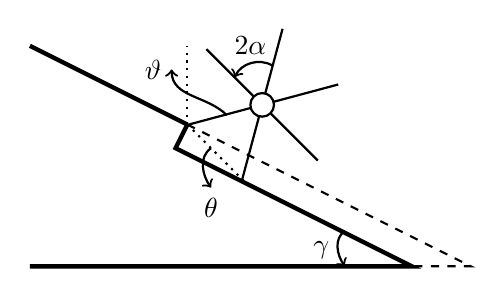
\begin{tikzpicture}
    \draw[-,ultra thick] (0,2) to (2,1);
    \draw[dashed, thick] (2,1) -- (5.6,-0.8)-- (4.85,-.8);
    \draw[ultra thick] (2,1) to (1.85,0.7) -- (4.85,-0.8)--(0,-0.8);
    \draw[thick] (2.95,1.25) circle (.15cm);
    \spoke{(2.95,1.25)}{-75};
    \spoke{(2.95,1.25)}{-15};
    \spoke{(2.95,1.25)}{45};
    \spoke{(2.95,1.25)}{105};
    \spoke{(2.95,1.25)}{165};
    \spoke{(2.95,1.25)}{-135};
    \draw[dotted,thick] (2,1) -- (2,2);
    \draw[dotted, thick] (2,1) -- (2.75,.25);
    \draw[->,thick] (2.3, 0.7) to [out=-145, in =125] (2.3,0.2) node[below] {$\theta$};
    \draw[->,thick] (4,-.35) to  [out=-145, in =125] (4,-0.8);
    \node at (3.7,-0.6) {$\gamma$};
    \draw[->, thick] (3.08,1.75) to [out=150, in =65] (2.6,1.6);
    \node at (2.8,2) {$2\alpha$};
    \draw[->,thick] (2.5,1.12) to [out=135, in =-90] (1.8,1.7) node[left]{$\vartheta$};
  \end{tikzpicture}
  \caption{Schematic of the rimless wheel with $\theta$ being the disturbance.}
  \label{fig:rw_schematic}
\end{figure}
\subsection{Problem description}
The objective of this work is to estimate the {\em largest set of initial conditions} from which all state trajectories of a hybrid quasi-uncertain system reach the terminal set $X_T$ in a pre-specified time, $T$.
\par
Depending on the edge set $\mathcal E$, there may be more than on trunk through which state trajectories can reach the terminal set. Consequently, the problem can be re-stated, with specificity, as wanting to find the largest set of initial conditions in each mode, $X_{(0,j)},\,\forall j\in \mathcal J$, that can reach $X_T$. That is, find $X_0$ where
%The projection of $\mathcal X_T$ onto each mode is the following
%$$\mathcal X_{T_j}=\{x\mid x\in \mathcal X_j\},\phantom{10}\forall j\in \mathcal J.$$
%\begin{assump}
%  $\mathcal X_{T_j},\,\forall j\in \mathcal J$, is a compact semi-algebraic set with bounding polynomials $h_{T_j}^i$, $i\in \N_{n_{h_T}^j}$.
%\end{assump}
%\begin{assump}
%The terminal set and guards are mutually exclusive; i.e.
%  $\forall \pi_{x}\left(\cup_{(i,j)\in \mathcal E}\,\mathcal G_{(i,j)}\right)\cap \mathcal X_T=\emptyset$.
%  \label{assump:guards_terminal}
%\end{assump}
$$X_0=\bigcup_{j\in \mathcal J} \mathcal X_{(0,j)},$$
and
\begin{align*}
\begin{aligned}
     X_{(0,j)}=\{y\in \mathrm M_j\mid x_0=y, x\colon [0,T]\rightarrow \cup_{i\in \mathcal J} \mathrm{M}_i,\\\,x(T)\in X_T \text{ using Alg.~\ref{alg:execution}}\}
\end{aligned}
\end{align*}
Observe that, by definition, for systems from $\mathfrak{U}$, if $X_{(0,j)}$ is the largest non-empty BRS in mode $j$, then all initial conditions from $X_{O0,j)}$, must reach $X_T$ at time $T$, regardless of the number of mode transitions that may occur in the interim and for every possible concomitant sequence of parametric uncertainty.
\par
For convenience, hereafter the times at which the system's state is relevant is denoted by the set $\mathcal T:=[0,\,T]$, and the projections of $X_T$ onto every mode, $j$, is denoted by $X_{(T,j)}$.

  \section{Problem Formulation}
\label{sec:prob}

In this section, we present a pair of dual infinite dimensional linear programs that compute the uncertain backwards reachable set.
Critically, note that despite the uncertainty being drawn from a distribution at the arrival into each mode, it remains constant throughout that mode.
As a result, this unknown parameter can be appended to the dynamics of every mode $j$ and treated as a portion of the state-space:
\begin{align}
f_j=\begin{bmatrix}
  \tilde f_j'&\mathbf{0}'_{n_{\theta_j}}
\end{bmatrix}'.
\end{align}
%In this augmented-state-space---henceforth referred to as the state-space of the system---the object of interest still remains the same, $X_{(0,j)},\,\forall j\in \mathcal J$. Furthermore, as the system transitions out of a mode, say at time $\tau_k$ the solution reaches $e_{ij}$, the uncertainty in mode $j$ is not related to the \emph{actual} value of the uncertainty in mode $i$ at $\tau_k$; in fact, the dimensions of the uncertain parameters $n_{\theta_j}$ need not equal $n_{\theta_i}$, much less their distributions.

To address this problem, we rely on the notion of occupation measures, first introduced in \cite{Pitman1977}, to transform the hybrid nonlinear dynamics of the system into a set linear dynamics over measures that can more readily be solved.
Occupation measures can be interested as measuring the time a solution spends in a portion of the state-space.
For instance, suppose the system enters mode $j$ at $\tau_k$ with the states being initialized as $x(\tau_k)=x_0$ and $\theta(\tau_k)=\theta$.
The occupation measure, \mbox{$\mu_j(\cdot\mid \tau_k,x_0,\,\theta)\in \mathcal M(\mathcal T\times D_j\times \Theta_j)$}, is defined as:

\small
\begin{align}
\hspace*{-1mm}\mu_j(A\times B\times C| \tau_k ,x_0,\theta)=\hspace*{-1.25mm}\int\limits_{\mathcal T} \hspace*{-1.25mm} I_{A\times B\times C}(t,x(t|\tau_k,x_0,\theta),\theta)dt.
\end{align}
\normalsize
Note the follow relation between the Lebesgue measure on $\mathcal T$ and $\mu_j(\cdot\mid \tau_k,x_0,\theta)$ holds for all $v \in C(\mathcal T\times D_j\times \Theta_j)$:
\begin{align}
\ip{\mu_j(\cdot\mid \tau_k,x_0,\theta),v}=\ip{\lambda_t,v(t,x(t\mid \tau_k,x_0,\theta),\theta)},
\label{eq:mu_lambda}
\end{align}
The occupational measure as defined is a conditional measure -- conditioned on the arrival-time and initial values of the states in that mode.
To consider a set of possible arrival-times and initial conditions, we define the \emph{average occupation measure} by integrating the conditional occupation measure against a measure on the set of possible initial conditions of the mode, $\mu_{s_j} \in  M(\mathcal T\times D_j\times \Theta_j)$:
\begin{align}
\mu_j(A\times B\times C)= \hspace*{-5mm}\int\limits_{\mathcal T\times D_j\times \Theta_j}\hspace*{-5mm}\mu_j(A\times B\times C\mid \tau_k,x_0,\theta)\,d \mu_{s_j}.
\label{eq:mu_avg}
\end{align}
Observe that by definition, the uncertain variables are independent of the states' initial conditions; hence $\mu_{s_i}\in \mathcal M(\mathcal T\times D_j\times \Theta)$ is expressible as a product measure:
\begin{align}
\mu_{s_j}=\bar\mu_{0_j}\otimes \mu_{\theta_j},\
\end{align}
where $\bar \mu_{0_j}\in \mathcal M(\mathcal T\times D_j)$ is a measure describing the set of initial conditions, and $\mu_{\theta_j}\in \mathcal M(\Theta_j)$ is as in the definition of $\mathcal H$.

Similarly, measures on terminals sets, $\mu_{T_j}\in \mathcal M(X_{(T,j)}\times \Theta_j)$:
\begin{align}
\mu_{T_j}(A\times B)= \hspace*{-4mm}\int\limits_{\mathcal T\times X_{(T,j)}\times \Theta_j}\hspace*{-4mm}I_{A\times B}(x(T\mid \tau_k,x_0,\theta),\theta)\,d\mu_{s_{j}},
\end{align}
and guards, $\mu_{ G_{(j,k)}}\in \mathcal M(\mathcal T\times  G_{(j,k)})$:
\begin{align}
\mu_{G_{(j,k)}}(A\times B\times C)=\hspace*{-5mm}\int\limits_{\mathcal T\times G_{(j,k)}}\hspace*{-5mm}I_{A\times B\times C}(t,x(t\mid \tau_k,x_0,\theta),\theta)\,d\mu_{s_{j}}
\end{align}
for all $(j,k) \in {\mathcal E}$ can be defined.
The measures $\mu_{ G_{(j,k)}}$ are supported on the guards of mode $j$ and should be interpreted as the hitting times of the guard.
The {\em final measure} in each mode $j$ can be defined as:
\begin{align}
  \mu_{f_j}=\delta_T\otimes \mu_{T_j}+\sum_{k\in\{l\mid (j,l)\in \mathcal E\}}\mu_{ G_{(j,k)}}.
\label{eq:mu_T}
\end{align}

% Given a set of initial conditions $X_{0}$, the dynamics of the system---under appropriate assumptions---defines a bundle of trajectories of the system states. It is of interest to ensure that this bundle terminates in the desired set $X_T$, making $X_0$ a subset of the BRS; stated differently, it is necessary to relate $\{\mu_{s_j}\}_{j\in \mathcal J}$ with $\{\mu_{f_j}\}_{j\in \mathcal J}$ and the dynamics of the system.
To compute $X_0$, we relate $\{\mu_{s_j}\}_{j\in \mathcal J}$ with $\{\mu_{f_j}\}_{j\in \mathcal J}$ using the dynamics of the system.
As a first step, define linear operators {$\mathcal L_{ f_j}\colon \mathcal C^1(\mathcal T\times D_j\times \Theta_j)\rightarrow \mathcal C(\mathcal T\times D_j\times \Theta_j)$} as:
\begin{align}
      \mathcal L_{f_j}v=\frac{\partial v}{\partial t}+\ip{\nabla_x v,\tilde f_j}
    \label{eq:Lv}
\end{align}
where $v\in \mathcal C^1(\mathcal T\times D_j\times \Theta_j;\R)$ is an arbitrary test function.
Suppose the system transitioned to mode $j$ at \mbox{$t=\tau_{k-1}$} with the state taking value upon reset $x(\tau_{k-1})$ and $\theta$.
The value of $v$, evaluated along the flow of the system and at $t=\tau_{k}$ is computed using the Fundamental Theorem of Calculus:
\begin{align}
\begin{aligned}
    v& \big(\tau_k,x(\tau_{k}\mid x(\tau_{k-1}),\theta_{k-1})\big)=v(\tau_{k-1},x(\tau_{k-1}),\theta_{k-1})\\
    &+\int_{\tau_{k-1}}^{\tau_{k}}\hspace*{-2mm}\mathcal L_{f}v(t,x(t\mid \tau_{k-1},x(\tau_{k-1}),\theta_{k-1}))\,dt.
\end{aligned}
\label{eq:FTC}
\end{align}
Using Eqn.~(\ref{eq:mu_lambda}), Eqn.~(\ref{eq:FTC}) can be re-written as:
\small
\begin{align}
\begin{aligned}
    v\big(\tau_k,&x(\tau_{k}\mid \tau_{k-1},x(\tau_{k-1}),\theta_{k-1})\big)=v(\tau_{k-1},x(\tau_{k-1}),\theta_{k-1})\\
    &+\ip{\mu_j(\cdot\mid \tau_{k-1},x(\tau_{k-1},\theta_{k-1}),\mathcal L_{ f}v},
\end{aligned}
\end{align}
\normalsize
which can be simplified further by using Eqns.~(\ref{eq:mu_avg})--(\ref{eq:mu_T}):
\begin{align}
  \ip{\mu_{f_j},v}=\ip{\mu_{s_j},v}+\ip{\mu_{j},\mathcal L_{f}v}.
  \label{eq:liouville_1}
\end{align}

Alternatively, using the standard definition of adjoint operators\footnote{A linear operator $\mathcal L$ and its adjoint, $\mathcal L'$, satisfy the following relation:
\begin{align*}
    \ip{\mathcal L'\mu,v}=\ip{\mu,\mathcal Lv}.
\end{align*}
% \begin{align*}
%     \ip{\mathcal L'\mu,v}=\ip{\mu,\mathcal Lv}=\int\limits_{\mathcal X}\mathcal Lv\,d\mu.
% \end{align*}
}, Eqn.~(\ref{eq:liouville_1}) is re-written as:
\begin{align}
\ip{\mu_{f_j},v}=\ip{\mu_{s_j},v}+\ip{\mathcal L'_{f}\mu_{j},v}.
  \label{eq:liouville_2}
\end{align}
\emph{Eqn~(\ref{eq:liouville_2}) defines a linear relation that initial and final measures evolving according to the hybrid dynamics must satsify.}


During the execution of a hybrid system, any mode can be entered either at $t=0$ or due to reset.
The initial measure in the $(t,x)$-coordinate can be decomposed as:
\begin{align}
  \bar\mu_{0_j}=\delta_0\otimes\mu_{0_j}+\pi^{(t,x)}_*\sigma_{0_j}
\end{align}
where $\mu_{0_j}\in \mathcal M(D_j)$ is the measure describing initial conditions to the system at $t=0$, $\sigma_{0_j}\in \mathcal M(\mathcal T\times D_j\times \Theta_j)$ is a measure describing initial conditions arriving due to reset, and $\pi^{(t,x)}_*$ denotes the pushforward constructed by lifting the $(t,x)$-projection operator, $\pi^{(t,x)}: \mathcal T\times D_j\times \Theta_j \to \mathcal T\times D_j$, to measures (refer to Chapter 11 in \cite{lee2003smooth} for an introduction to pushforwards).
State resets occur when the state reaches a guard.
As a result, we must formalize a relationship between $\mu_{ G_{(i,j)}}$ and $\sigma_{0_j},~\forall (i,j)\in \mathcal E$.
To formalize this relationship notice that $\sigma_{0_j}$ can be decomposed into measures corresponding to the source of each arrival state:
\begin{align}
  \sigma_{0_j}=\sum_{i\in \{k\mid (k,j)\in \mathcal E\}} \sigma_{(i,j)}\otimes \mu_{\theta_j},
\end{align}
where $\sigma_{(i,j)}$ is the measure describing initial conditions that are reset into mode $j$ from guard $G_{(i,j)}$.
Upon reaching the guard, the system transitions according to the reset map, $R_{(i,j)}$, which can be treated as a nonlinear transformation between $D_i$ and $D_j$.
By applying a change of variables formula, as in Lemma 1 in \cite{shia2014convex}, we have:
\begin{align}
    \ip{\sigma_{(i,j)},w}=\ip{\pi^{(t,x)}_*\mu_{ G_{(i,j)}},w\circ R_{(i,j)}}
    \label{eq:reset_measure}
\end{align}
where $w\in \mathcal C(\mathcal T\times \mathcal D_j)$ and
$$
  \ip{\pi_{t,x}\mu_{ G_{(i,j)}},s}=\ip{\mu_{ G_{(i,j)}},s},\,\forall s\in \mathcal C(\mathcal T\times D_i);
$$
essentially, $\sigma_{(i,j)}$ is a push-forward measure of $\mu_{ G_{(i,j)}}$.
%\begin{remark}
%\label{remark:primal}
%  \red{A note on domain in time and the Liouville's equations}
%\end{remark}
  \subsection{The primal}
  \label{ssec:primal}
  With the constraints expressed in terms of measures, the problem of approximating the BRS is formulated as an infinite-dimensional Linear Program that supremizes the \emph{volume} of the set of initial condition.
  \begin{flalign}\nonumber
  &\sup_{\Lambda}\sum_{j=1}^{n_m}\ip{\mu_{0_j},1}&&&(P)\\\nonumber
  &\text{st.}\\
  &\mu_{s_j}+\mathcal L_{f}'\mu_j=\,\mu_{f_j}&&&\forall j\in \N_{n_m}\label{eq:primal:liouville}\\
  &\mu_{0_j}+\hat\mu_{0,j}=\,\lambda_j&&&\forall j\in \N_{n_m}\\
  &\sum_{j=1}^{n_m}\ip{\mu_{T_j},1}=\,\sum_{j=1}^{n_m}\ip{\mu_{0_j},1}\label{eq:mass_conservation}
  \end{flalign}
  where $\lambda_j$ is the Lebesgue measure supported on $D_j$.
  $$\Lambda=\{\mu_j,\mu_{0_j},\mu_{T_j},\hat\mu_{0_j},\mu_{ G_{(j,k)}}\ge 0,\,\forall j\in \mathcal \N_{n_m},(j,k)\in \mathcal E\}.$$
Variables $\hat\mu_{0_j}\in \mathcal M(D_j)$ are slack variables introduced to enforce a stronger constraint than absolute continuity of $\mu_{0_j}$ wrt. to $\lambda_j$
  \begin{flalign}
  &&&\mu_{0_j}(A)\le \lambda_j(A)&\forall A\subset D_j\label{eq:primal:domination}
    \end{flalign}
  The constraint in Eqn.~(\ref{eq:mass_conservation}) ensures that all trajectories that emanate $\cup_{j\in \mathcal J}\,spt(\mu_{0_j})$ reach $X_{T}$ at $t=T$, and is not {\em stuck} at any of the guards.
  %%%%%%%%%%
  \begin{lemma}
   If $\mu_{0_j},\forall j\in \mathcal J$ is part of the optimal solution of ($P$) then $\bigcup_{j\in \mathcal J}\,spt(\mu_{0_j})$ is the BRS of the system. In addition, the optimal value of ($P$) is equal to $\sum_{j\in \mathcal J}\lambda_j(X_{0_j})$, the sum of \emph{volumes} of the BRSs in each mode.
  \end{lemma}

  \begin{proof}
  Suppose $\sum_{j\in \mathcal J}\lambda_j(spt(\mu_{0_j})\backslash X_{(0,j)})>0$, then by Lemma~\ref{lemma:existence}, there exist trajectories that begin in $\cup_{j\in \mathcal J}(spt(\mu_{0_j})\backslash X_{(0,j)})$ that reach $X_T$; this is a contradiction. Thus,
  \begin{align}
  &\bigcup_{j\in \mathcal J} spt(\mu_{0_j})\subset \bigcup_{j\in \mathcal J} X_{(0,j)},\\
  &\sum_{j\in \mathcal J}\lambda_j(spt(\mu_{0_j}))\le\sum_{j\in \mathcal J}\lambda_j( X_{(0,j)}).
  \label{eq:support_lemma:1}
  \end{align}
    By definition of the BRS, all state trajectories that emanate from a subset of $X_0$ end in $X_T$. That is, for each $j\in \mathcal J$ and initial measure $\mu_{0_j}$, if $spt(\mu_{0_j})\subset X_{(0,j)}$, there exist measures $\mu_{j}$ and $\mu_{f_j}$ that satisfy Eqn.~(\ref{eq:primal:liouville}). Thus the following inequality is true.
    \begin{align}
    \sum_{j\in \mathcal J}\lambda_j(spt(\mu_{0_j}))\ge \sum_{j\in \mathcal J}\lambda_j(X_{(0,j)})
      \label{eq:support_lemma:2}
    \end{align}
   From Eqns.~(\ref{eq:support_lemma:1})\&(\ref{eq:support_lemma:2}), $\cup_{j\in \mathcal J}\,spt(\mu_{0_j})$ is the BRS of the system.
    \par
    That the optimal value of $(P)$ is volume of the BRS follows from Eqn.~(\ref{eq:primal:domination}) and the observation that \mbox{$\lambda_{j}|_{X_{(0,j)}},\forall j\in \mathcal J$} is feasible in ($P$).
  \end{proof}

  \subsection{The dual}
  \label{ssec:dual}
    The dual corresponding to $(P)$ is derived using standard techniques and is presented below.
    \par
    \footnotesize
    \begin{flalign}\nonumber
    &&&\inf \sum_{j\in \N_{n_m}}\ip{\lambda_j,w_j}&(D)\\\nonumber
    &&&\text{st.}\\
    &&&w_j\ge \,0&\forall j\in \mathcal J\\
    &&& v_j(T,\cdot)+q\ge\, 0 ,\> &\forall (j,x,\theta)\in \mathcal J\times X_{(T,j)}\times \Theta_j \label{eq:dual:terminal}\\
    &&& - \mathcal L_{f}v_j\ge\,0 ,\> &\forall j\in \mathcal J\label{eq:dual:lfv}\\
    &&& w_j-\ip{\mu_{\theta_j},v_j(0,\cdot)}-q\ge \,1 ,\> &\forall j\in \mathcal J\label{eq:dual:levelset}\\
    &&&v_j\ge\, \ip{\mu_{\theta_k},v_k}\circ R_{(j,k)},&\forall (j,k,x,\theta)\in \Upsilon\label{eq:dual:mode_transition}
    \end{flalign}
    \normalsize
    where $q\in \R$, $v_j\in C^1(\mathcal T\times \mathrm M_j\times \Theta_j)$ and $w_j\in C(\mathrm M_j)$ $\Upsilon=\mathcal J\times G_{(j,k)}\times \mathcal E$.
    \begin{lemma}
      If $(w,v,q)$ is the solution to (D), then the super-level set
      \begin{align}
      \bigcup_{j\in \mathcal J}\,\{x\mid w_j(x)\ge 1\}
      \end{align}
      is an outer approximation of the BRS of the system whose dynamics is described by Alg.~\ref{alg:execution}.
      \label{lemma:dual_outerapprox}
    \end{lemma}
    \begin{proof}
    The approach we adopt to prove this lemma is to construct the projection of the BRS on any mode and show that it is a 1-level set of the appropriate function. To assist in constructing the arguments, assume wlog., that the state trajectory terminates in $X_{(T,j_k)}$ for some $j_k$. The state trajectory must have arrived in mode $j_k$ through a finite sequence of mode-transitions (according to Assumption~\ref{assump:zeno}); wlog., let this sequences of mode-transitions be of length $k$. Suppose the states entered mode $j_k$ at time $\tau_k$, then, from the fundamental theorem of calculus and the constraints in Eqns.~(\ref{eq:dual:terminal})\&(\ref{eq:dual:lfv}), the following inequalities follow.
    \begin{align}
      -q\le v_{j_k}(T,x(T\mid x(\tau_k^+),\theta),\theta)\le v_j(\tau_k,x(\tau_k^+),\theta)\\
      \Rightarrow -q\le \ip{\mu_{\theta_{j_k}},v_{j_k}(\tau_k,x(\tau_k^+),\theta)}
    \end{align}
    By iterative application of the constraint in Eqn.~(\ref{eq:dual:mode_transition}) and finally Eqn.~(\ref{eq:dual:levelset}), it follows that
    \begin{align}
      -q\le&\, \ip{\mu_{\theta_{j_k}},v_{j_k}(t,x,\theta)}\circ R_{(j_{k-1},j_{k})}(\tau_{k},x(\tau_{k}^-))\\
      \le&\, v_{j_{k-1}}(\tau_{k},x(\tau_{k}^-\mid x(\tau_{k-1}^+),\theta),\theta)\\
      \le &\, \ip{\mu_{\theta_{j_{k-1}}},v_{j_k}(\tau_k,x(\tau_{k-1}^+),\theta)}\\\nonumber
      &\,\vdots\\
      \le &\,v_{j_0}(\tau_1,x(\tau_1^-\mid x_0,\theta),\theta)\\
      \le &\,v_{j_0}(0,x_0,\theta)\\
      \le &\,\ip{\mu_{\theta_{j_0}},v_{j_0}(0,x_0,\theta)}\\
      \le &\, w_{j_0}(x_0)-q-1.
    \end{align}
    The final inequality implies that for every trajectory that ends in $X_{(t,j_k)}$, $x(t)=x_0\in D_{j}$  satisfies the condition $w_{x_0}\ge 1$. Thus the set of initial conditions that begin in mode $j_0$ and reach the terminal set projected into mode $j_k$ is given by the super-level set
    \begin{align}
      I_{(j_0,j_k)}=\{x\mid w_{j_0}\ge 1\}.
    \end{align}
    Note that the definition of $I_{j_0,j_k}$ does not depend on the mode in which the terminal set is reached; thus \mbox{$I_{(j_0,\mathcal J)}=X_{(0,j_0)}$}. Finally, by observing that $j_0$ is an arbitrary element of $\mathcal J$, we deduce the stated result.
    \end{proof}
    \begin{lemma}
      There is not gap between (P) and (D).
    \end{lemma}
    \begin{proof}
      The proof follows from \cite[Theorem 3.10]{Anderson1987}, and is similar to \cite[Theorem 2]{henrion2014convex}; it is not presented for brevity.
    \end{proof}
    \begin{remark}
    There are two key aspects of the presentation in this section that deserve re-iteration: (1) by definition, the uncertainties that influence the dynamics can be visualized as a discrete random process with updates to the instantiation of the uncertainty occurring upon entering a new mode; (2) the estimated BRS is the set of initial conditions from which {\em all} trajectories that emanate reach the terminal set for {\em all} possible discrete sequence of uncertainty. As a direct implication of the second point, the solution of the problem is the intersection of the BRS of every possible sequence of uncertainty.
    \end{remark}

  \section{Numerical Implementation}
\label{sec:implementation}

In this section, a sequence of Semidefinite Programs (SDP)s that approximate the solution to the infinite dimensional primal and dual defined in Secs.~\ref{ssec:primal} and \ref{ssec:dual} are introduced.
This sequence of relaxations is constructed by characterizing each measure using a sequences of moments\footnote{The $n$th moment of a measure ($\mu$) is obtained by evaluating the following expression
  $$y_{\mu,n}=\ip{\mu,x^n}.$$}
and assuming the following:
\begin{assump}
The vector field in each mode and reset map between modes is a polynomial. 
Moreover the domain, the value of uncertainties, the guard, and the target set in each mode is a semi-algebraic set.
  \label{assump:poly}
\end{assump}
Recall that polynomials are dense in the set of continuous functions by the Stone-Weierstrass Theorem so this assumption is made without too much loss of generality.

Under this assumption, given any finite $d$-degree truncation of the moment sequence of all measures in the primal $(P)$, a primal relaxation, $(P_d)$, can be formulated over the moments of measures to construct an SDP. 
The dual to $(P_d)$, $(D_d)$, can be expressed as a sums-of-squares (SOS) program by considering $d$-degree polynomials in place of the continuous variables in $D$.

To formalize this dual program, first note that a polynomial $p \in \R[x]$ is SOS or $p \in \text{SOS}$ if it can be written as $p(x) = \sum_{i=1}^m q_i^2(x)$ for a set of polynomials $\{q_i\}_{i=1}^m \subset \R[x]$.
Note efficient tools exist to check whether a finite dimensional polynomial is SOS using SDPs~\cite{parrilo2000structured}.
Next, suppose we are given a semi-algebraic set $A = \{x \in \R^n \mid h_{i}(x) \geq 0, h_i \in \R[x], \forall i \in \N_m \}$.
We define the $d$-degree {\em quadratic module} of $A$ as:
\begin{align}
  \begin{split}
  Q_d(A)=\bigg\{q\in \R_d[x]\,\bigg|\, \exists \{s_k\}_{k \in N_m \cup \{0\}} \subset \text{SOS s.t. } \\ q=s_0+\sum_{k\in \N_{m}}h_{k}s_k \bigg\}
  \end{split}
\end{align}

\noindent The $d$-degree relaxation of the dual, $D_d$, can be written as:
  \begin{flalign}\nonumber
    & & \inf_{\Xi_d} \hspace*{0.1cm} & \sum_{j\in \mathcal J}\int_{D_j}w_j(x)\,d\lambda_j(x) && \hspace*{-0.3cm} (D_d) \nonumber\\
    & & \text{st.} \hspace*{0.1cm} & w_j^d\in Q_d(X_{(T,j)}) && \hspace*{-0.3cm} \forall j\in \mathcal J \nonumber\\
    & & & v_j^d(T,\cdot)+p\in Q_d(D_{j} \times \Theta_j) && \hspace*{-0.3cm} \forall j\in \mathcal J \nonumber\\
    & & & -\mathcal L_{f_j}v_j^d\in Q_d(\mathcal T\times D_{j} \times \Theta_j) && \hspace*{-0.3cm} \forall j\in \mathcal J \nonumber\\
    & & & w_j^d-\ip{\mu_{\theta_j},v_j^d(0,\cdot)}-p-1\in Q_d(D_j) && \hspace*{-0.3cm} \forall j\in \mathcal J \nonumber\\
    & & & v_j^d-\ip{\mu_{\theta_k},v_k^d}\circ R_{(j,k)}\in Q_d(\mathcal T \times D_j \times \Theta_j) && \hspace*{-0.3cm} \forall (j,k)\in {\cal E} \nonumber
  \end{flalign}
where $\Xi_d=\Big\{ \big(\{v^d_j\}_{j\in {\cal J}},\{w^d_j\}_{j \in {\cal J}},p \big) \in \bigtimes_{j\in {\cal J}}\R_d[t,x,\theta]$ $\bigtimes_{j \in {\cal J}} \R_d[x]\times\R \Big\}$.
A primal can similarly be constructed, but the solution to the dual can be used directly generate a sequence of outer approximations to the uncertain backwards reachable set:
\begin{lemma}
	For each $d \in \N$ and $j \in {\cal J}$, let $w_{j_d}$ denote the $j$-slice of the $w$-component of the solution to $D_d$. Then ${\cal X}_{(0,j_d)} = \{x \in D_j \mid w_{j_d}(x) \geq 1 \}$ is an outer approximation to ${\cal X}_{(0,j)}$ and $\lim_{d\to\infty}\lambda_{n_j}({\cal X}_{(0,j_d)} \backslash {\cal X}_{(0,j)}) = 0$.
\end{lemma}
\begin{proof}
  The proof to this lemma is an extension of Theorems 5--7 in \cite{shia2014convex} given Lemma \ref{lemma:dual_outerapprox}.
\end{proof}

    \section{Implementation and Examples}
  In this section, the efficacy of the proposed method is evaluated through three examples. The relaxed problems were parsed using the SPOTLESS toolbox and were numerically solved using MOSEK on a computer equipped with a Intel Xeon W3540 processor and 12GB of RAM.
  The following points on the examples considered are obligatory.
  \begin{enumerate}
    \item It is a characteristic trait of the problem formulation considered in this paper that the actual distribution of the uncertainty is immaterial. Consequently, in all examples, it is assumed that the disturbance is uniformly distributed.
    \item For reasons related to numerics, all problems are normalized such that the state-space is given by $[-1,1]^n$, for an appropriate value of $n$.
  \end{enumerate}
  Also, since has been established that the solution of relaxed problems provides an outer approximation of the BRS, in this section, the qualifier `approximate' is suppressed.
  \subsection{1-D linear dynamics}
  The first example under consideration is that of a one-state system whose dynamics is described by
  \begin{align}
	\dot x =&\, -0.7x+0.2\theta-0.1,
    \label{eq:ex:1}
\end{align}
where $\theta$ is an uncertain parameter. Note that this system is not a hybrid system; however, by setting $n_m=1$ and using identity reset maps, the dynamics can be hybridized. In the implementation whose results are depicted in Fig.~\ref{fig:1D:linear}, the guard is set at $x=1$ and the degree relaxation, $d=12$.
\begin{figure}[!t]
  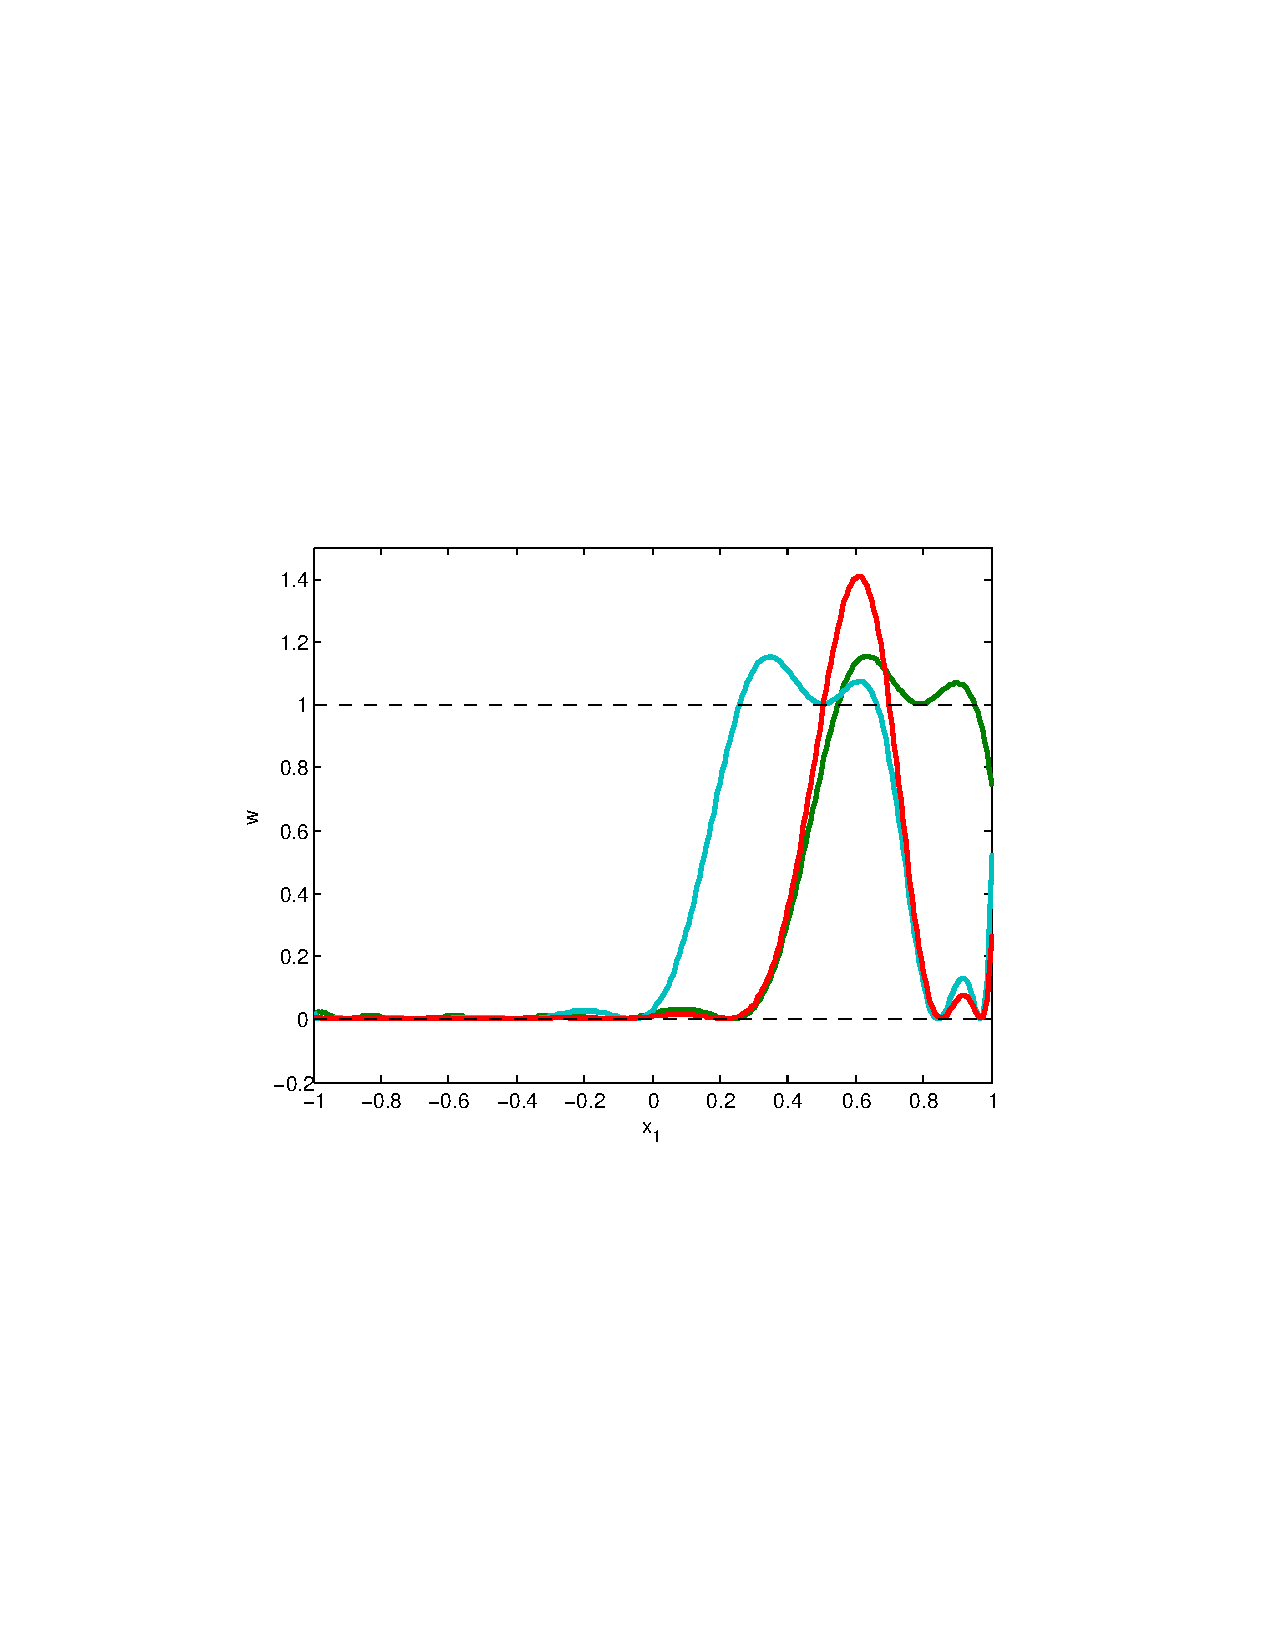
\includegraphics[width=\columnwidth,trim =1.5in 3.3in 1.5in 3.5in, clip=true]{figures/1D_3}
  \caption{Outer approximations of the BRS of the extreme deterministic cases and the stochastic case.(green) $\theta=0$, (blue) $\theta=1$ and (red) $\mu_\theta$}
    \label{fig:1D:linear}
\end{figure}
\par
Figure~\ref{fig:1D:linear} presents the graph of $w_1^{12}$ computed for each of the following cases -- (1) $\theta=0$ (green), (2) $\theta=1$ (cyan), and (3) $\theta\in \mathcal U(0,1)$ (red); when the terminal time is $T=1$ and the terminal set is $\mathcal X_T=[0.2,0.4]$. Observe that the BRS corresponding to case (3) encloses the intersection of those of cases (1) and (2); this is the desired outcome.
\subsection{Rimless wheel}
The planar rimless wheel---constituted by a massless axle to which $n$ equidistant (angular) spokes are connected---is one of the simplest models of legged locomotion. Figure~\ref{fig:rw_schematic} presents a schematic of a rimless wheel---with spokes separated by an angle $2\alpha$---rolling down an infinite wedge. The dynamics of this rimless wheel between transitions is described by
$$
  \begin{bmatrix}
    \dot \theta& \ddot\theta
  \end{bmatrix}'=\begin{bmatrix}
    \dot\theta&\sin(\theta)
  \end{bmatrix}',
$$
where $\theta$ is the angle between the pivoted spoke and the vertical. Once the marching spoke makes contact with the terrain, the states are reset using the maps
$$
  \begin{bmatrix}
    \theta^+&&
    \dot \theta^+
  \end{bmatrix}'=\begin{bmatrix}
    2\gamma-\theta^-&
    \cos(2\alpha)\,\dot\theta^-
  \end{bmatrix}'.
$$
\begin{figure}[!t]
\centering
  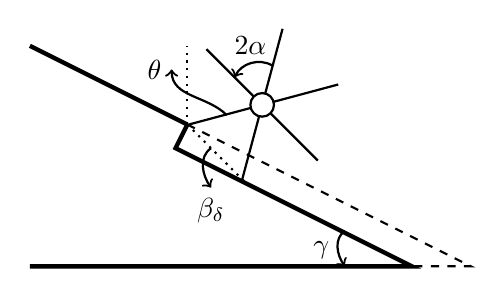
\begin{tikzpicture}
    \draw[-,ultra thick] (0,2) to (2,1);
    \draw[dashed, thick] (2,1) -- (5.6,-0.8)-- (4.85,-.8);
    \draw[ultra thick] (2,1) to (1.85,0.7) -- (4.85,-0.8)--(0,-0.8);
    \draw[thick] (2.95,1.25) circle (.15cm);
    \spoke{(2.95,1.25)}{-75};
    \spoke{(2.95,1.25)}{-15};
    \spoke{(2.95,1.25)}{45};
    \spoke{(2.95,1.25)}{105};
    \spoke{(2.95,1.25)}{165};
    \spoke{(2.95,1.25)}{-135};
    \draw[dotted,thick] (2,1) -- (2,2);
    \draw[dotted, thick] (2,1) -- (2.75,.25);
    \draw[->,thick] (2.3, 0.7) to [out=-145, in =125] (2.3,0.2) node[below] {$\beta_\delta$};
    \draw[->,thick] (4,-.35) to  [out=-145, in =125] (4,-0.8);
    \node at (3.7,-0.6) {$\gamma$};
    \draw[->, thick] (3.08,1.75) to [out=150, in =65] (2.6,1.6);
    \node at (2.8,2) {$2\alpha$};
    \draw[->,thick] (2.5,1.12) to [out=135, in =-90] (1.8,1.7) node[left]{$\theta$};
  \end{tikzpicture}
  \caption{Schematic of the rimless wheel with $\beta_\delta$ being the disturbance.}
  \label{fig:rw_schematic}
\end{figure}
In this example, it is assumed that the slope (terrain) is not flat and that the relative depth of the next step is $\delta$; this translates to an angle $\beta_\delta$ relative to the slope of the wedge. The disturbance to the dynamics of the rimless wheel, $\beta_\delta$, manifests itself in the guard of the only mode in this hybrid system. The angle at which the marching spoke lands on the surface satisfies
$$
  \theta=\gamma+\alpha+\beta_\delta.
$$
An analytically computable stable limit cycle for the disturbance-free rimless wheel exits []; however, for the case considered in this example, the definition of a limit cycle less clear. Consequently, a notion of {\em meta-stability}---when the system states arrive within $\epsilon$ of the stable limit cycle of the disturbance-free system---is adopted.
\par
Figure~\ref{fig:rw_brs} presents the degree 12 BRS (black dashed) for the rimless wheel (with $\alpha=0.4$) which is tasked with arriving within the red band in $T=4$ seconds, as it is rolling down a wedge with slope $\gamma=0.2$ withstanding an a sequence of random changes to terrain drawn from $\beta_\delta\sim\mathcal U([-0.1,0.1])$. The relative depths/height of the disturbance is about 25\% the length of each spoke.
\par
The BRS is validated by performing Monte Carlo simulations; the box $I^2$ is discretized into 51 points both ways and 100 independent trajectories are simulated (using MATLAB's ode45 function) from each initial condition. The blue $\times$s depict the initial conditions that arrived within the terminal set at the desired time without violating any of the other constraints. Note that the set of points that succeeded in the MC simulation is entirely contained in the BRS.
\begin{figure}[!t]
  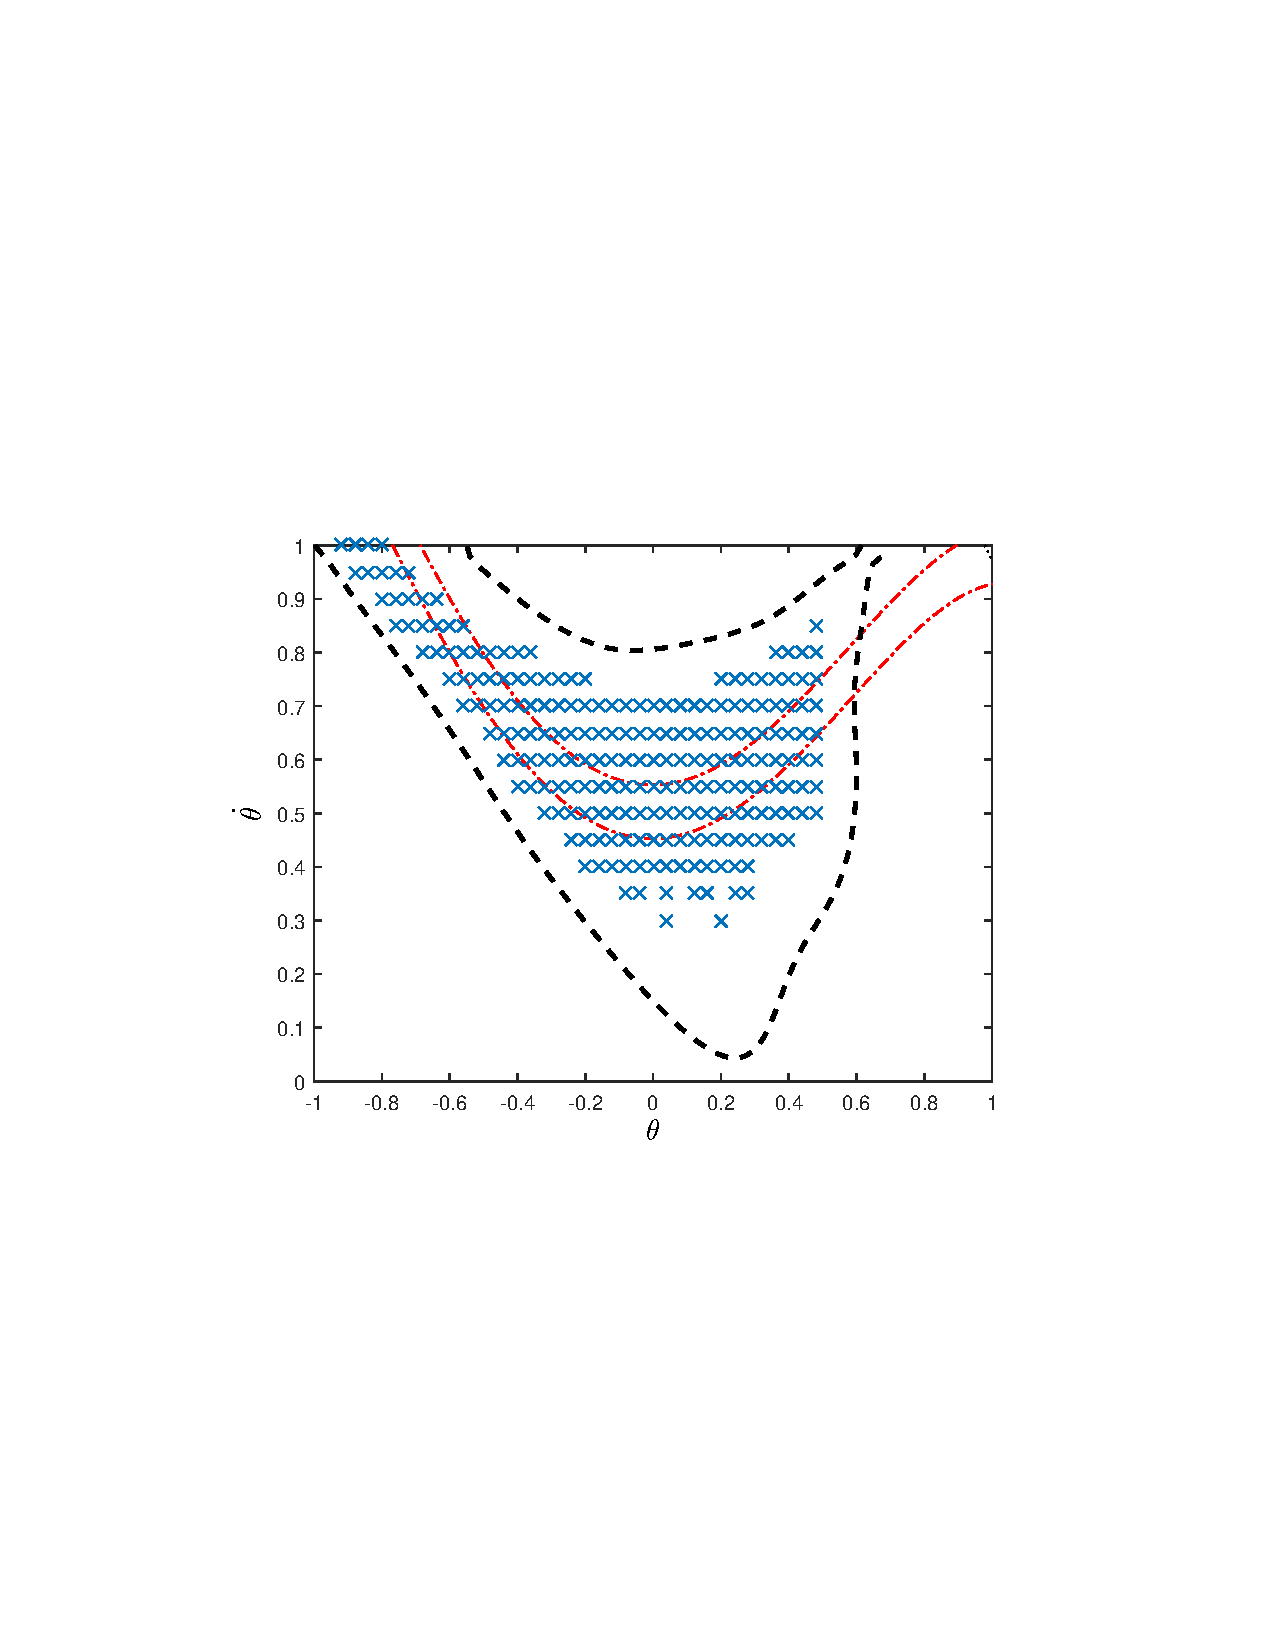
\includegraphics[trim=1.5in 3.3in 1.5in 3.5in, clip=true,width=\columnwidth]{figures/rw_0p1_4}
  \caption{Outer approximation and estimated BRS based on 100 iterations and T=4. Red band is the terminal set and the black outer is the boundary of the estimated BRS; the crosses correspond to results of MC simulation.}
  \label{fig:rw_brs}
\end{figure}
\par
At this juncture, a remark about the tightness of the BRS is warranted. Clearly, the BRS in Fig.~\ref{fig:rw_brs} is not tight; and we attribute this to the set of basis functions with which are currently working--monomials; and the degree relaxation. As commented in [], adopting an alternate basis set is likely to increase the rate of convergence and the tightness. As it stands, there are alternate ways to improve the tightness, primary amongst which is to create phantom modes using identity reset maps; this approach however, needs some care and is deferred for a future work.

  \section{Conclusions}
In this paper, a convex approximation of the reachable sets of a class of uncertain polynomial hybrid drift systems is presented. The presented method optimizes over the set of unsigned measures using converging moment relaxations and SDPs. A commentary on the accuracy and the adequacy of the proposed method is provided using examples. A future work will extend the work herein by synthesizing \emph{cautious} feedback control laws that guarantee constraint satisfaction. 
  \appendix
  \section{Existence of solutions}
  \begin{lemma}[Existence of solutions]
Let $(\mu_{s_j},\mu_{f_j},\mu_j), j\in \mathcal J$ satisfy Eqn.~(\ref{eq:primal:liouville}). Then, there exists a family of absolutely continuous trajectories starting from $\mu_{s_j}$ such the occupation and final measures in each mode generated by this family of trajectories is equal to $\mu_j$ and $\mu_{f_j}$.
    \label{lemma:existence}
  \end{lemma}
%
%  \begin{proof}[Proof (sketch)]
%  Given the cyclical definition of systems in $\mathfrak{U}$, it suffices to show that solutions exists in any one mode; wlog., let us consider mode $j$. In addition, wlog. let the time when the trajectory is begins in the support of $\check\mu_{0_j}$ be $\tau$. To assist in the ensuing presentation, define the dynamics of the system in mode $j$ as the following
%  \begin{align}
%    \bar f_j(x,\theta)=\begin{cases}
%      \tilde f_j(x,\theta)& (x,\theta)\not\in \bigcup\limits_{k\in \{l\mid (j,l)\in \mathcal E\}}\mathcal G_{(j,k)}\\
%      0& \text{o.w.}
%    \end{cases}
%  \end{align}
%    If the beginning time in mode $j$ is $\tau$, by Lemma 3 in \cite{henrion2014convex}, given the above dynamics, there exists a family of trajectories that reaches $\mu_{f,j}$. Trajectories that reach a guard before $t=T$, and get stuck would be reset and the system enters another mode wherein similar arguments can be used to show the existence of absolutely continuous trajectories.
%  \end{proof}

\bibliographystyle{ieeetr}
\bibliography{references,refs}
\end{document}
